\documentclass[a4paper,11pt]{article}
\usepackage{lecturenotes}
\usepackage{float}
\lectureheader{ELE734}{2}
\begin{document}
\tableofcontents
\clearpage
\notesection{Cross-section of a Inverter}

The sizing of a CMOS device takes up actual real estate on the silicon and introduces trade-offs such as capacitance, resistance etc. Furthermore, in a CMOS device, the PMOS device has twice the width of the NMOS device.

\begin{figure}[htbp]
    \centering
    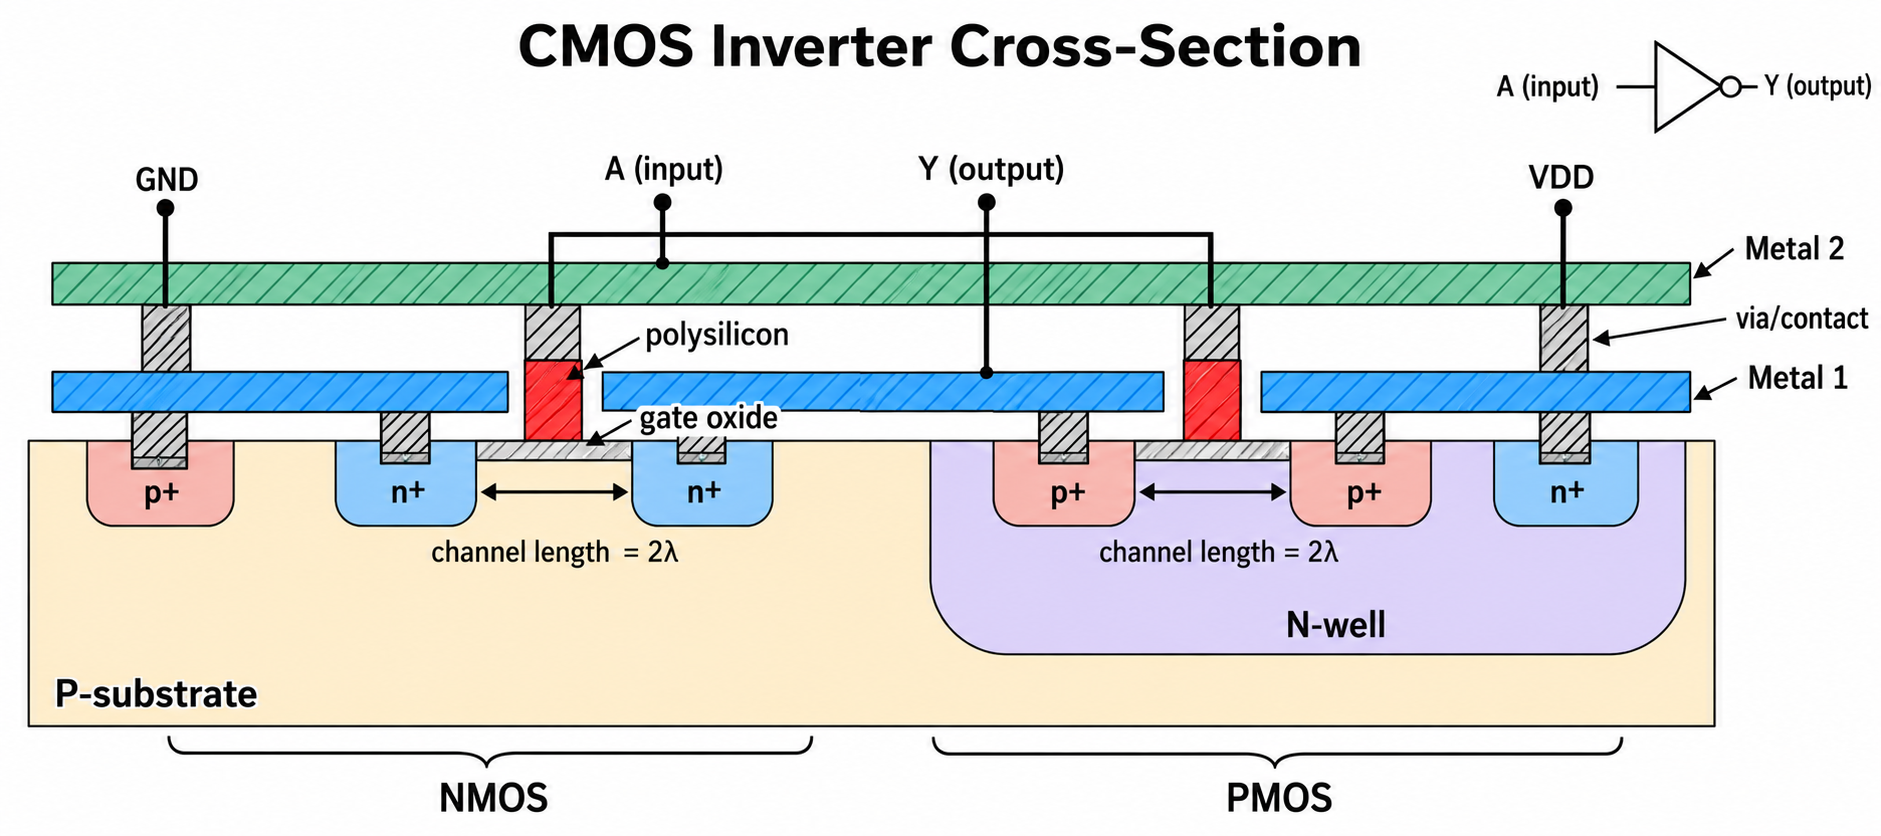
\includegraphics[width=1\linewidth]{figures/cmos-inverter-cross-section.png}
    \caption{CMOS-Inverter Cross Section}
    \label{fig:}
\end{figure}

\notesection{Layout Design Rules}

Due to the secrecy regarding most silicon processes, in order to standarize design rules, a \textbf{$\lambda$-based} approach is used instead
\notedefinition{$\lambda$-based Design Rules for Planar Layout}{
    \[
        \begin{aligned}
            \lambda
             & = \frac{1}{2}\cdot\text{Channel Length}                      \\
             & = \frac{1}{2}\cdot\text{Minimum width of a polysilicon wire}
        \end{aligned}
    \] \\
    \textcolor{red}{*} All design rules are based on \textbf{integer multiples} of $\lambda$. Therefore in a 180nm process, lambda would be defined as: $\lambda = 90nm$
}

\begin{notetable}
    {>{\arraybackslash}p{0.18\linewidth} >{\centering\arraybackslash}p{0.30\linewidth} >{\centering\arraybackslash}X}
    {\textbf{Layer} & \textbf{Minimum Rules} & \textbf{Reference}}
    \begin{minipage}[c]{\linewidth}
        \bfseries Metal
    \end{minipage}
    & \begin{minipage}[c]{\linewidth}
        \centering
        \begin{tabular}{@{}l@{\hspace{1.5em}}c@{}}
            Width   & $4\lambda$ \\
            Spacing & $4\lambda$
        \end{tabular}
    \end{minipage}
    & \begin{minipage}[c]{\linewidth}
        \centering
        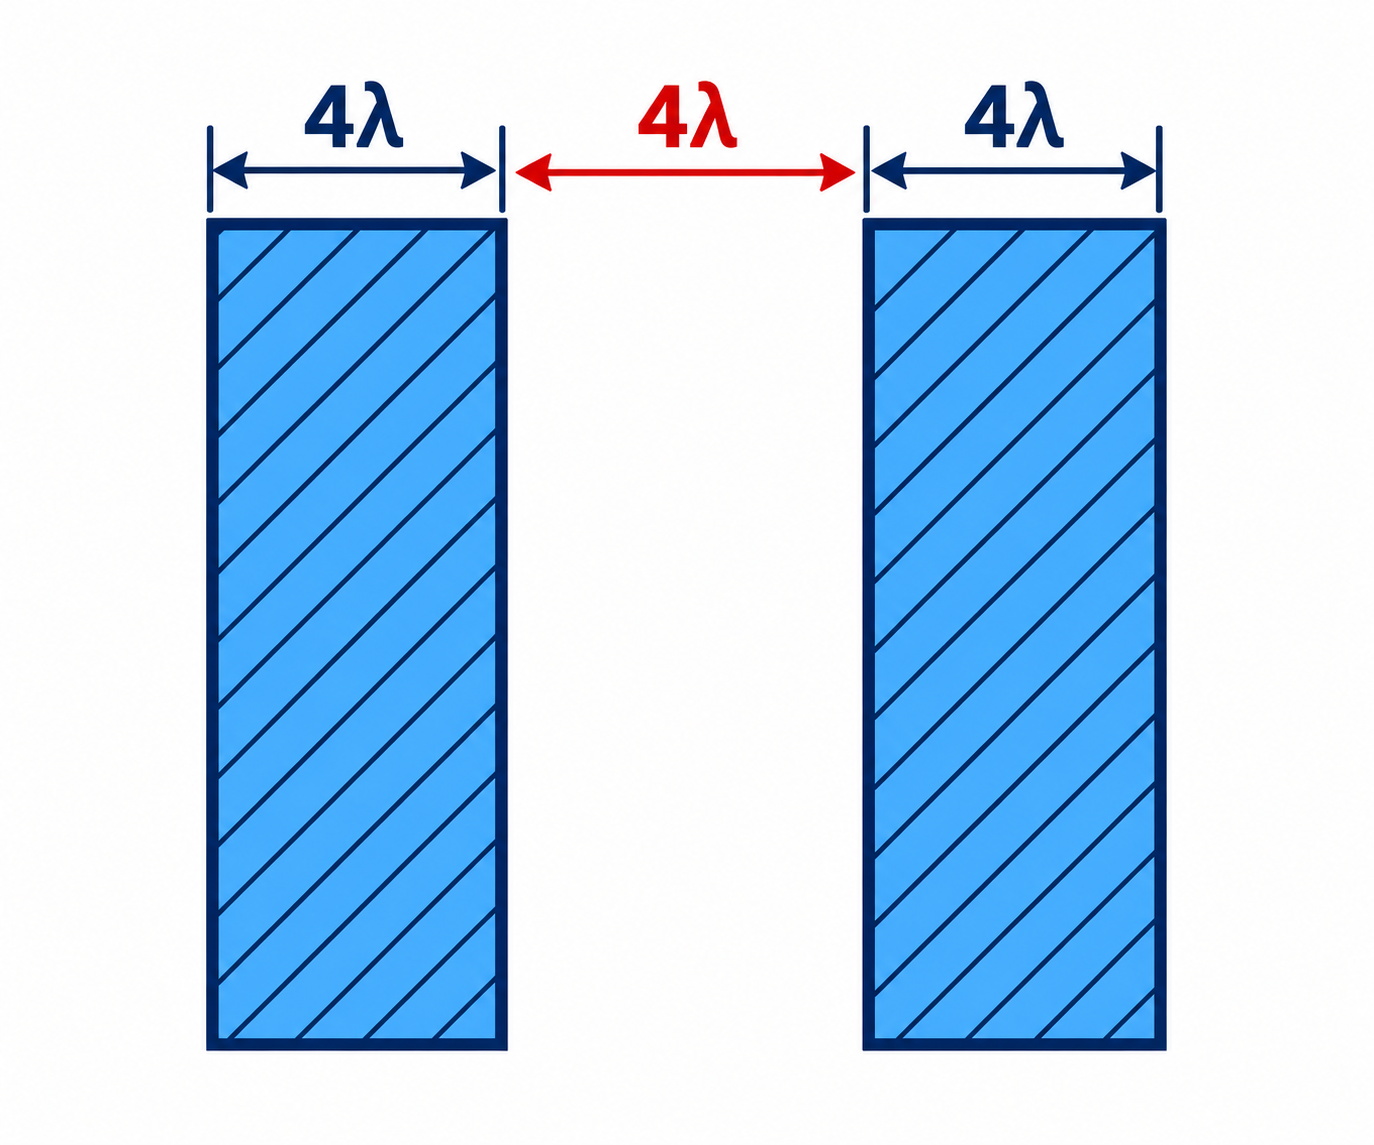
\includegraphics[height=28mm,width=0.9\linewidth,keepaspectratio]{figures/lambda-metal-width-spacing.png}
    \end{minipage} \\
    \midrule
    \begin{minipage}[c]{\linewidth}
        \bfseries Diffusion
    \end{minipage}
    & \begin{minipage}[c]{\linewidth}
        \centering
        \begin{tabular}{@{}l@{\hspace{1.5em}}c@{}}
            Width   & $4\lambda$ \\
            Spacing & $4\lambda$
        \end{tabular}
    \end{minipage}
    & \begin{minipage}[c]{\linewidth}
        \centering
        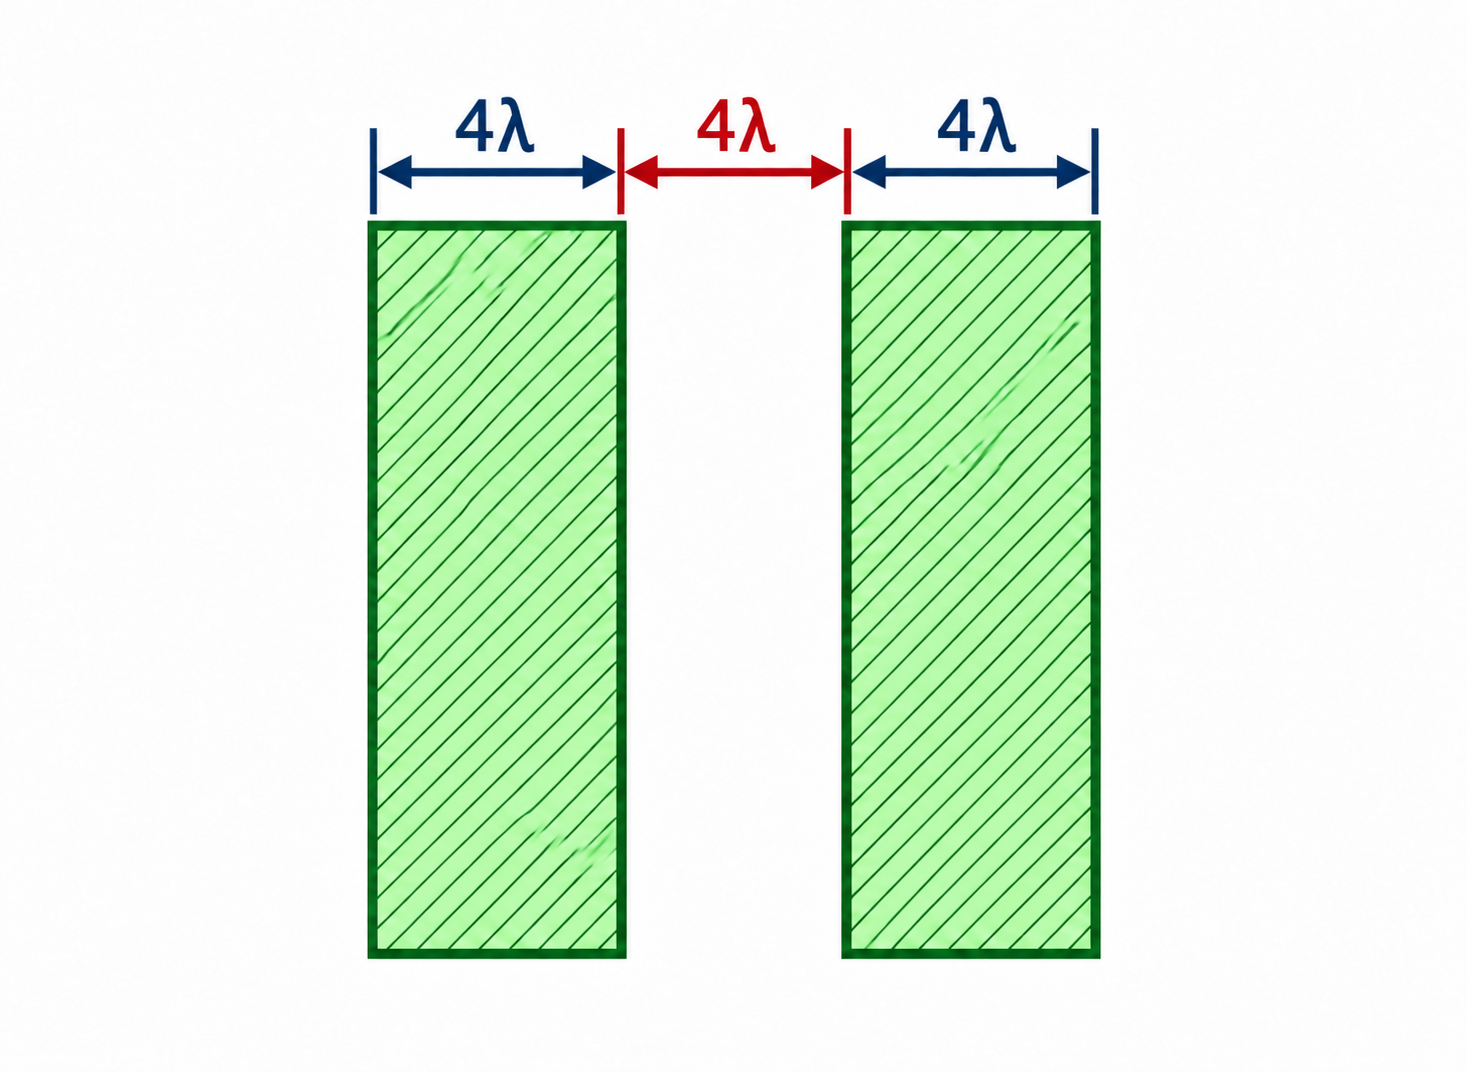
\includegraphics[height=28mm,width=0.9\linewidth,keepaspectratio]{figures/lambda-diffusion-minimum-width.png}
    \end{minipage} \\
    \midrule
    \begin{minipage}[c]{\linewidth}
        \bfseries Polysilicon
    \end{minipage}
    & \begin{minipage}[c]{\linewidth}
        \centering
        \begin{tabular}{@{}l@{\hspace{1.5em}}c@{}}
            Width   & $2\lambda$ \\
            Spacing & $3\lambda$
        \end{tabular}
    \end{minipage}
    & \begin{minipage}[c]{\linewidth}
        \centering
        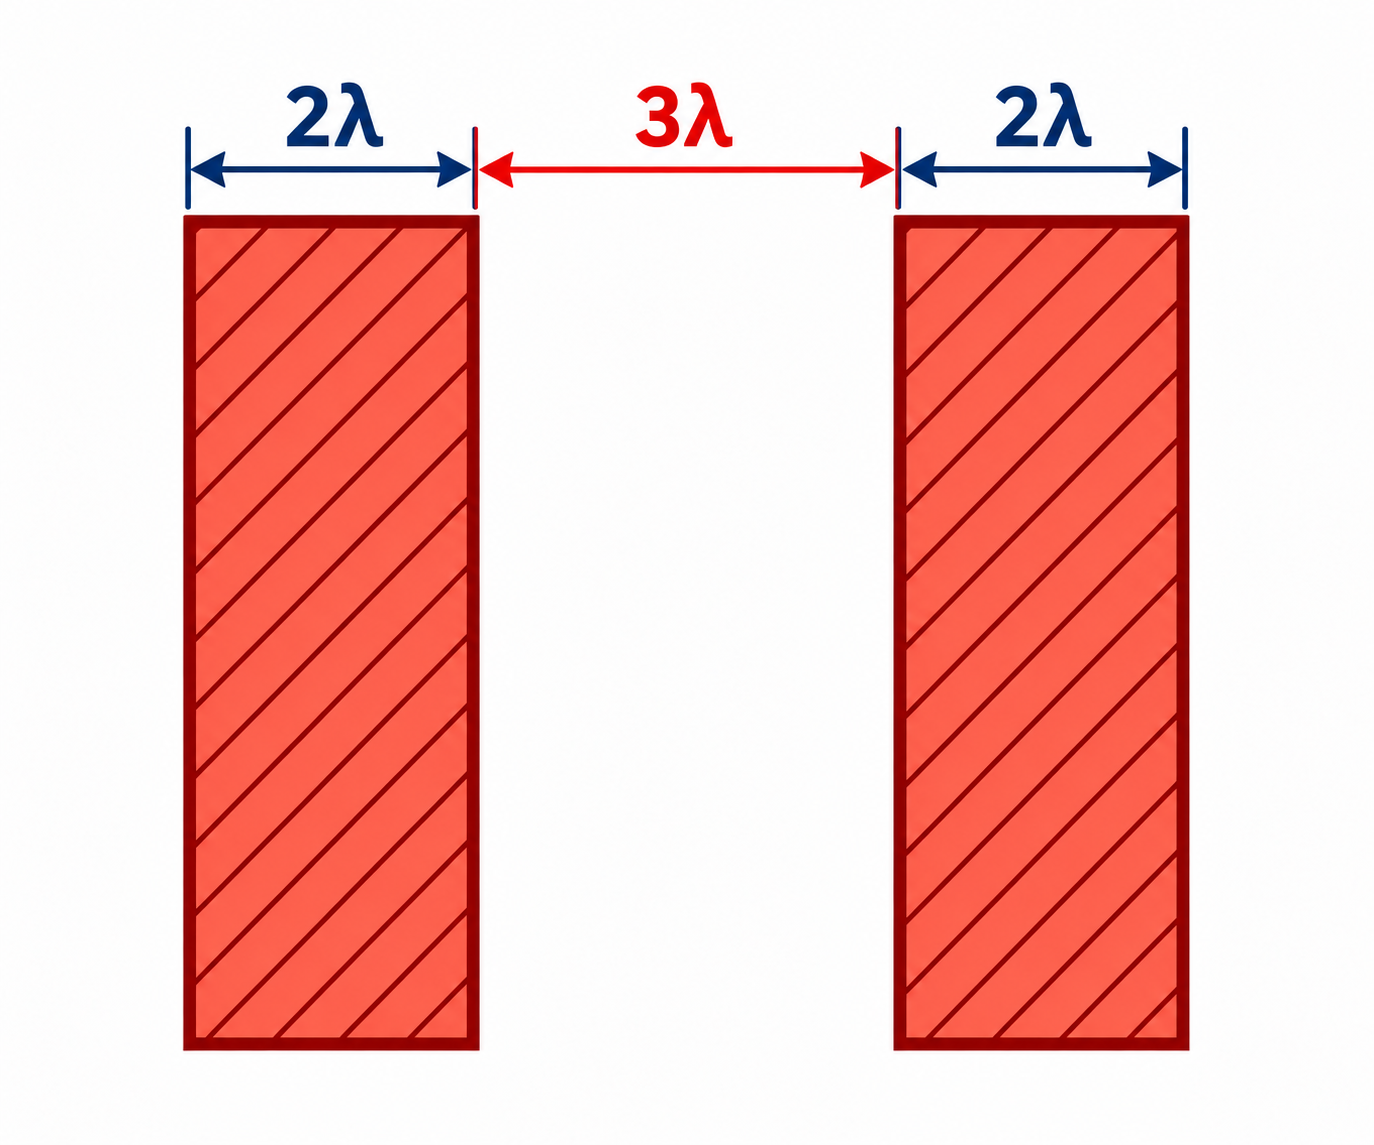
\includegraphics[height=28mm,width=0.9\linewidth,keepaspectratio]{figures/lambda-polysilicon-width-spacing.png}
    \end{minipage} \\
    \midrule
    \begin{minipage}[c]{\linewidth}
        \bfseries Contact/via
    \end{minipage}
    & \begin{minipage}[c]{\linewidth}
        \centering
        \begin{tabular}{@{}l@{\hspace{1.5em}}c@{}}
            Opening  & $2\lambda \times 2\lambda$ \\
            Surround & $4\lambda \times 4\lambda$
        \end{tabular}
    \end{minipage}
    & \begin{minipage}[c]{\linewidth}
        \centering
        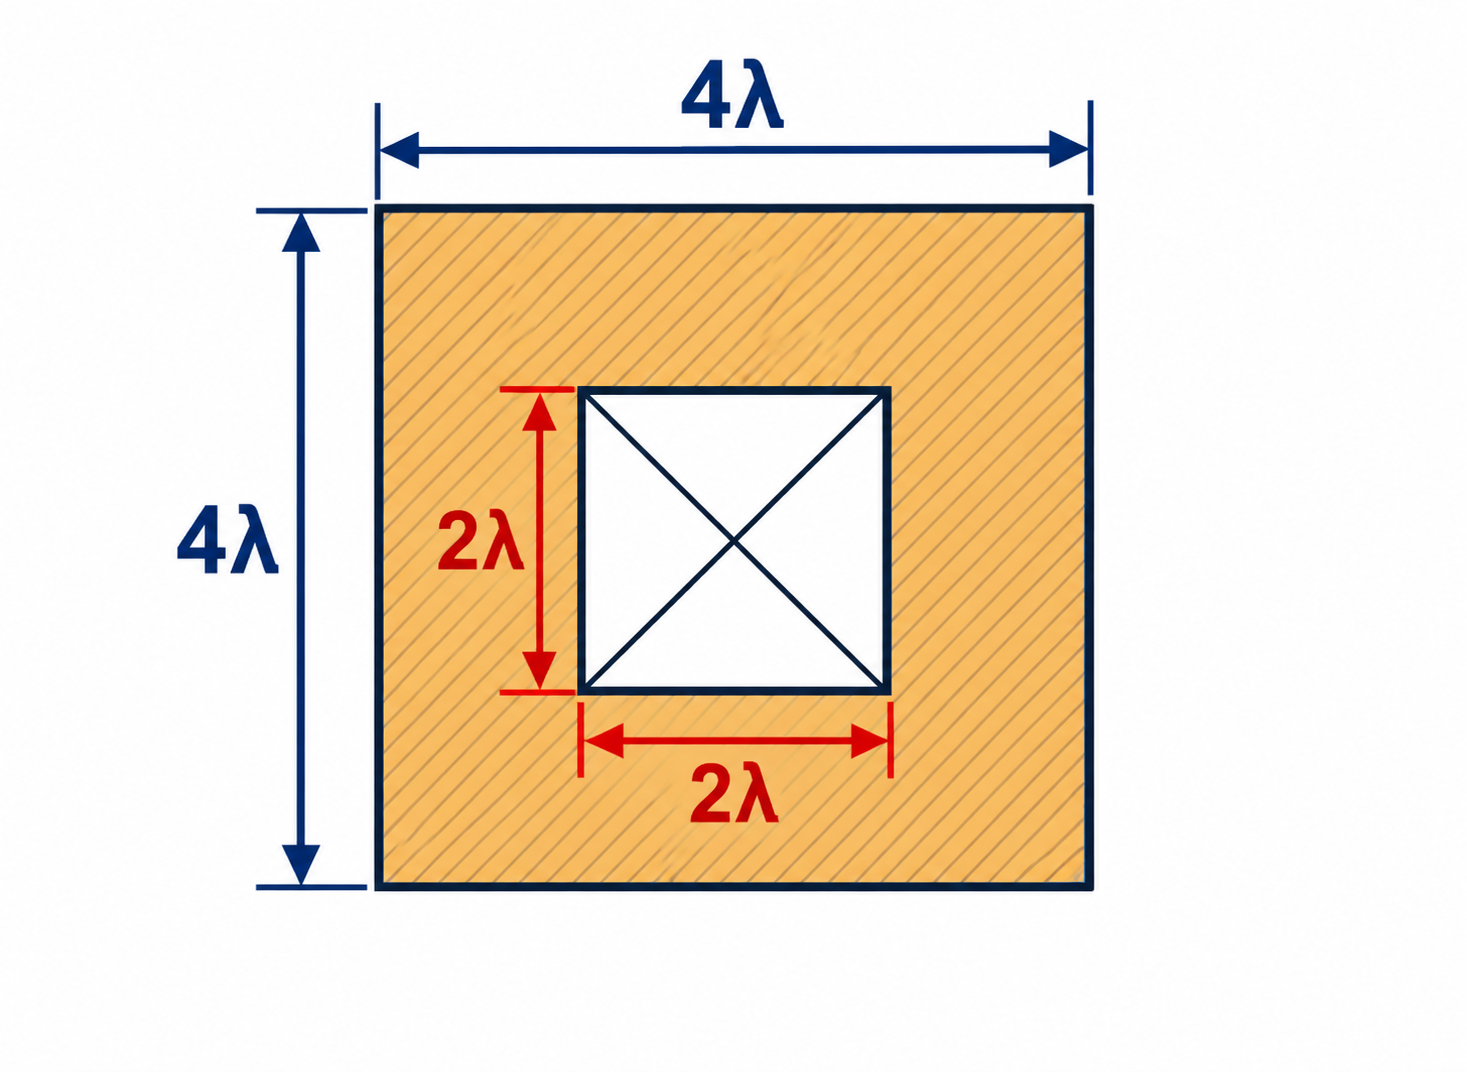
\includegraphics[height=28mm,width=0.9\linewidth,keepaspectratio]{figures/lambda-contact-via-dimensions.png}
    \end{minipage} \\
    \midrule
    \begin{minipage}[c]{\linewidth}
        \bfseries P/N-wells
    \end{minipage}
    & \begin{minipage}[c]{\linewidth}
        \centering
        \begin{tabular}{@{}l@{\hspace{1.5em}}c@{}}
            Active to well edge & $6\lambda$
        \end{tabular}
    \end{minipage}
    & \begin{minipage}[c]{\linewidth}
        \centering
        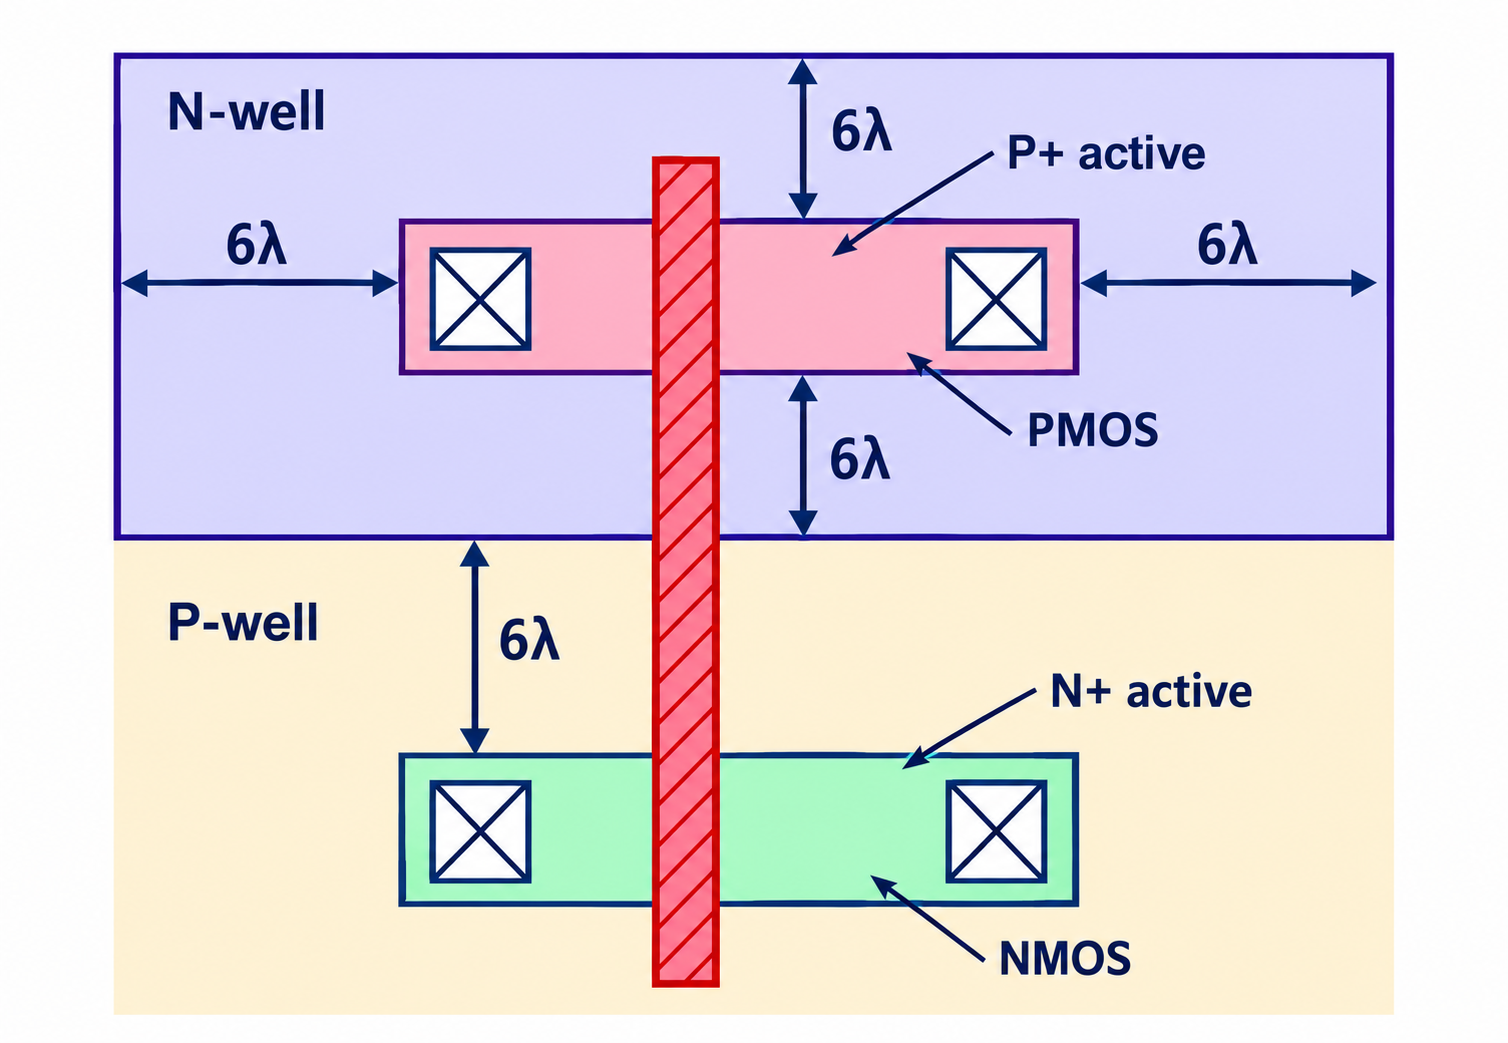
\includegraphics[height=28mm,width=0.9\linewidth,keepaspectratio]{figures/lambda-nwell-pwell-separation.png}
    \end{minipage} \\
\end{notetable}

So for an actual transistor layout we would have something like:
\begin{figure}[htbp]
    \centering
    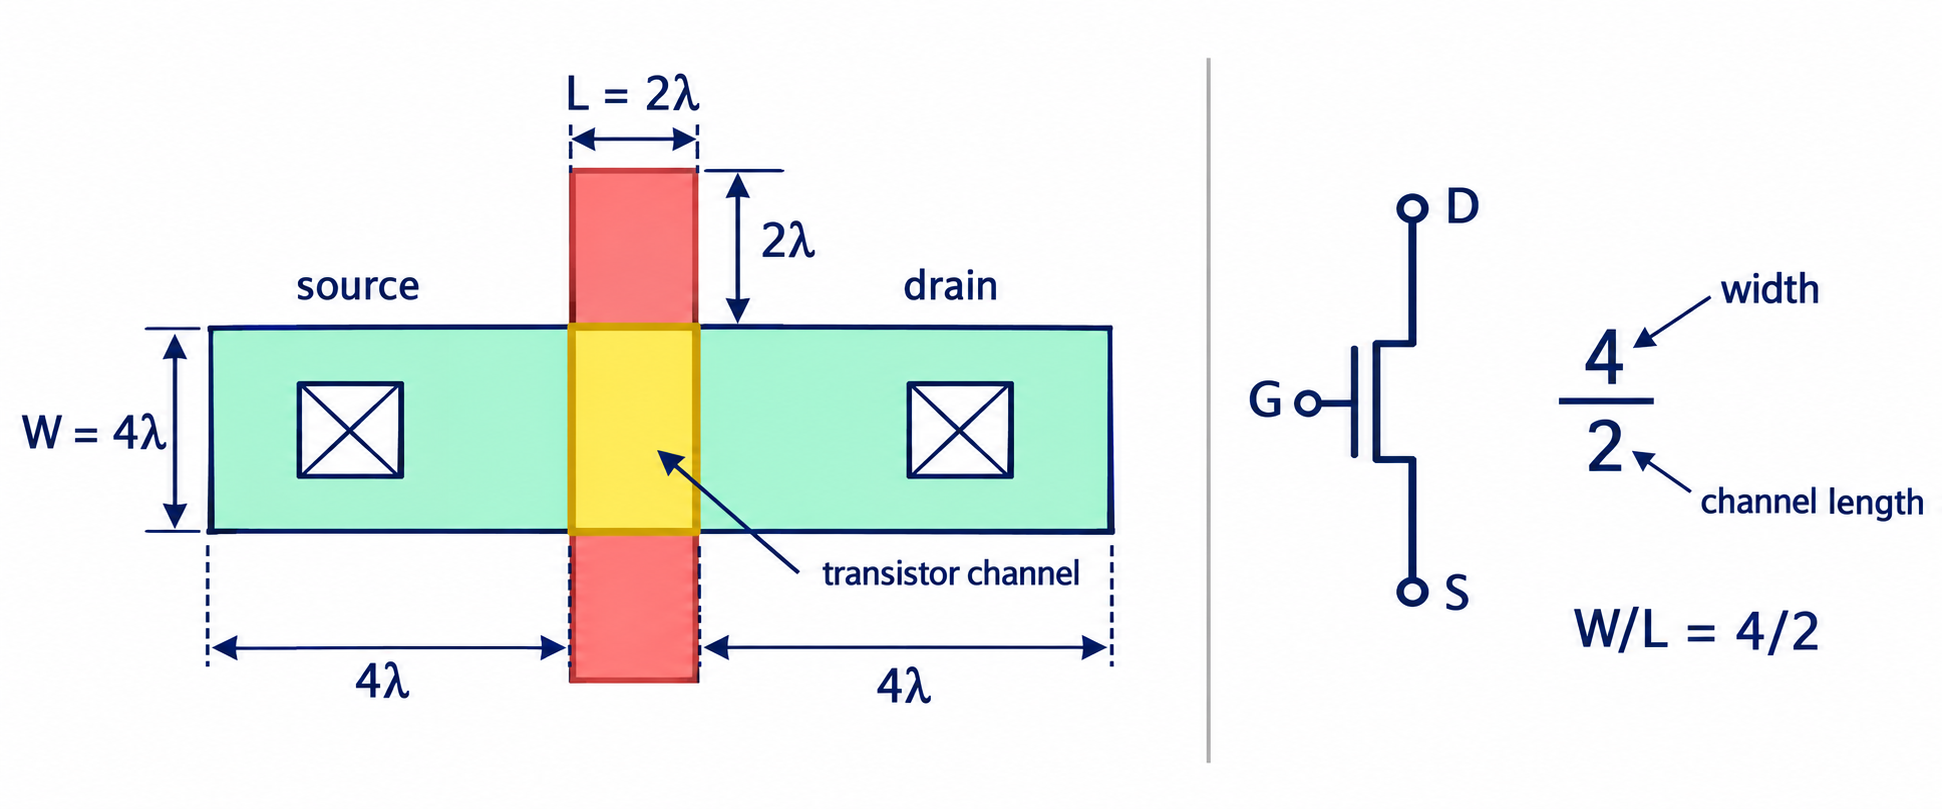
\includegraphics[width=0.8 \linewidth]{figures/lambda-transistor-layout-symbol.png}
    \caption{Unit Transistor Layout}
    \label{fig:}
\end{figure}

The true length of the transistor would be: $12\lambda$, the true width: $4\lambda$ therefore its area would be approximately: $8\times12\lambda^2$. If we were to double the width of the transistor, we would find the area to only have increased by $1.5x$, while the drive strength would be doubled.

\notedefinition{Transistor Layout}{
    \begin{itemize}
        \item The above figure is known as the \textcolor{red}{unit transistor}
        \item In layout, the length is never made bigger as it usually always has an unwanted effect on the devices properties
    \end{itemize}
}

\notesection{Stick Diagram Layout \& Area Estimation}
\subnotesection{Laying Out a Cell in Standard Cell Design}

\begingroup
\setlength{\intextsep}{4pt}
\setlength{\abovecaptionskip}{6pt}
\begin{figure}[htbp]
    \centering
    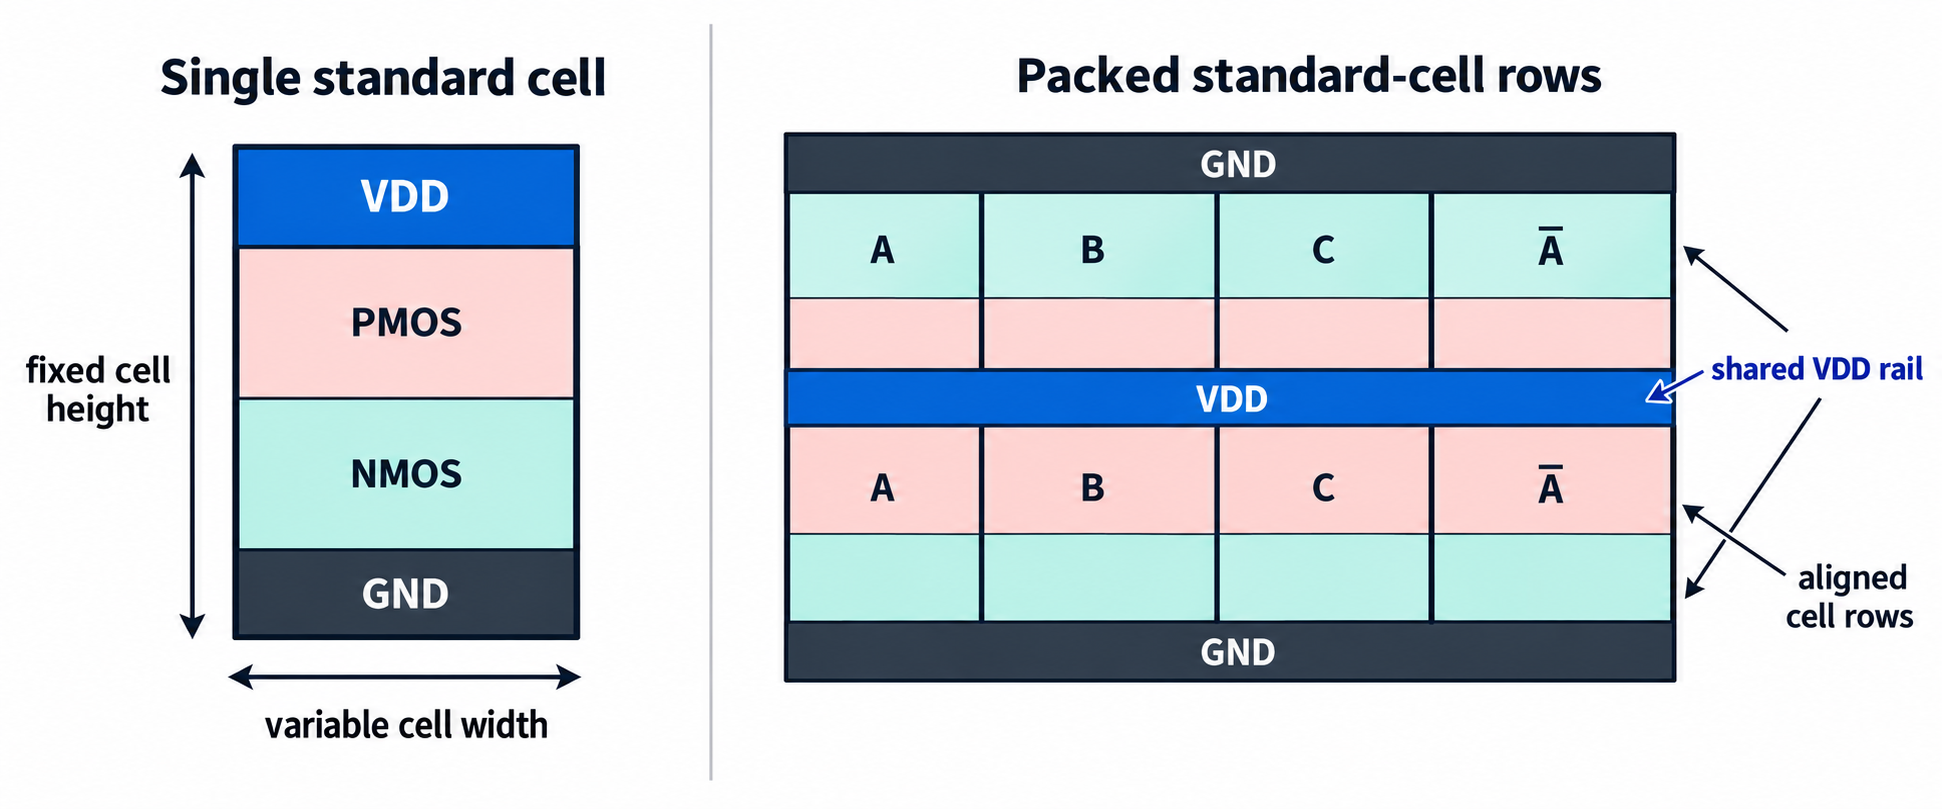
\includegraphics[width=0.8\linewidth]{figures/standard-cell-structure-and-row-packing.png}
    \caption{Standard Cell Structure \& Row Packing}
    \label{fig:}
\end{figure}

\noindent\begin{minipage}[t]{\linewidth}
\subnotesection{Stick Diagram for an Inverter}

\begin{figure}[H]
    \centering
    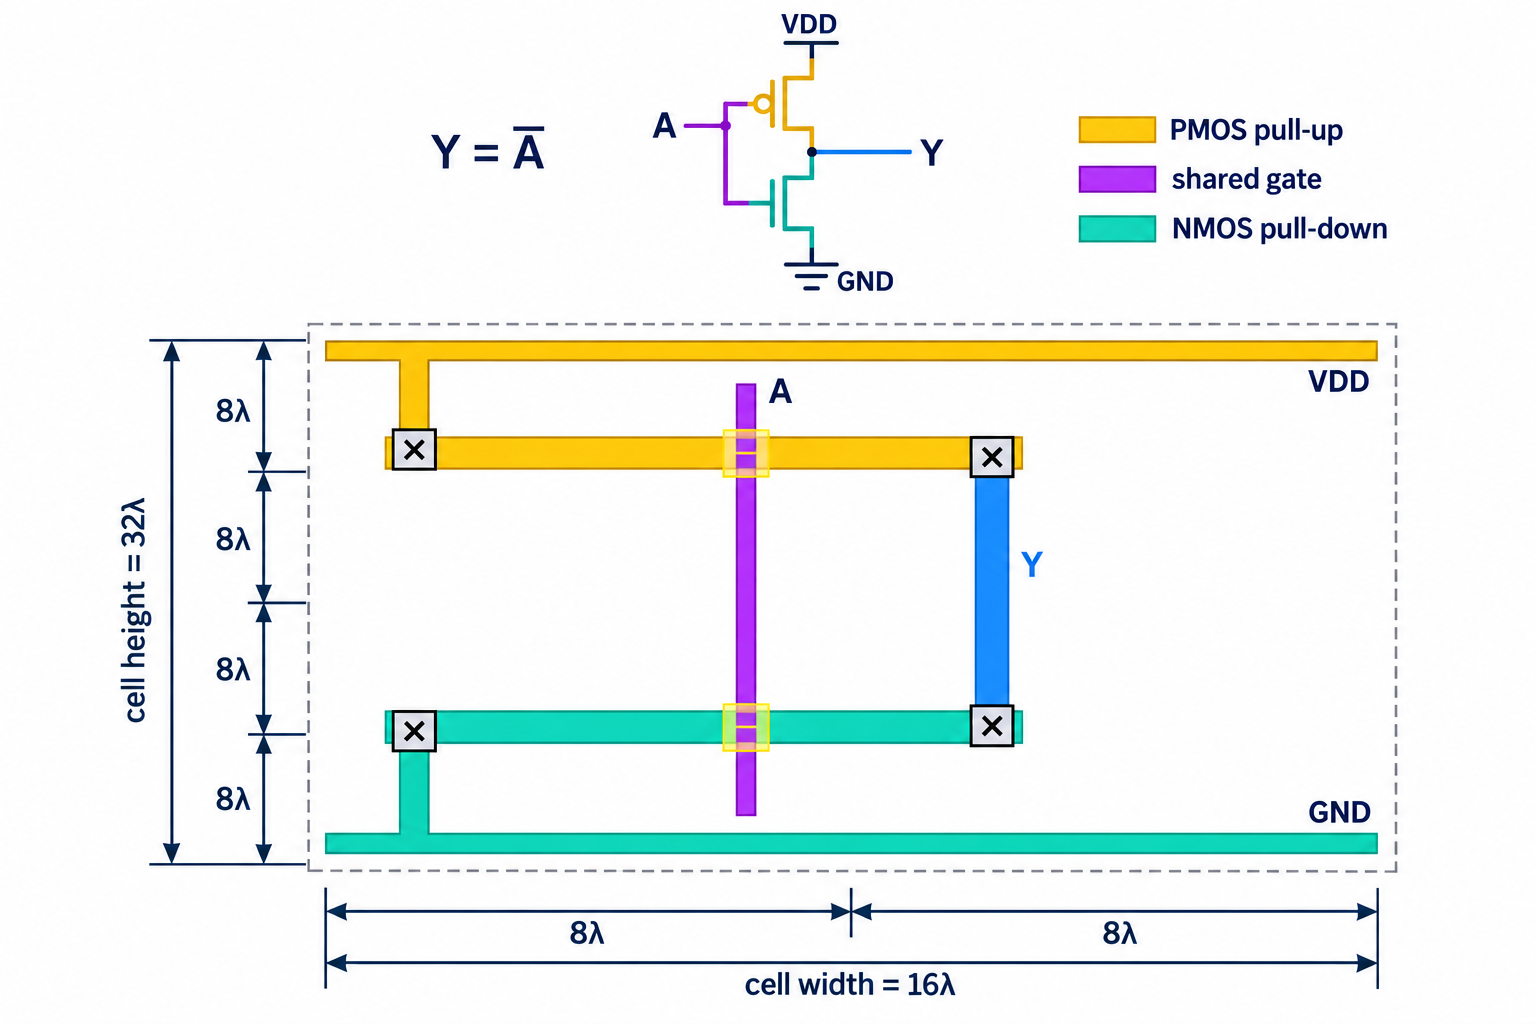
\includegraphics[width=0.65\linewidth]{figures/inverter-stick-diagram-area-estimation.png}
    \caption{Inverter Stick Diagram for Area Estimation}
    \label{fig:}
\end{figure}
By summing the corresponding widths and lengths we find the area of the inverter to be: $A \approx 32 \lambda \times 16 \lambda = 512 \lambda$
\end{minipage}\par
\endgroup

\notebox{Important Rule}{
    There \textcolor{red}{should be \textbf{NO} unneccessary} diffusion breaks. Meaning that S\&D should be shared across neighboring transistors to minimize and standardize layout area.
}

\begin{figure}[htbp]
    \centering
    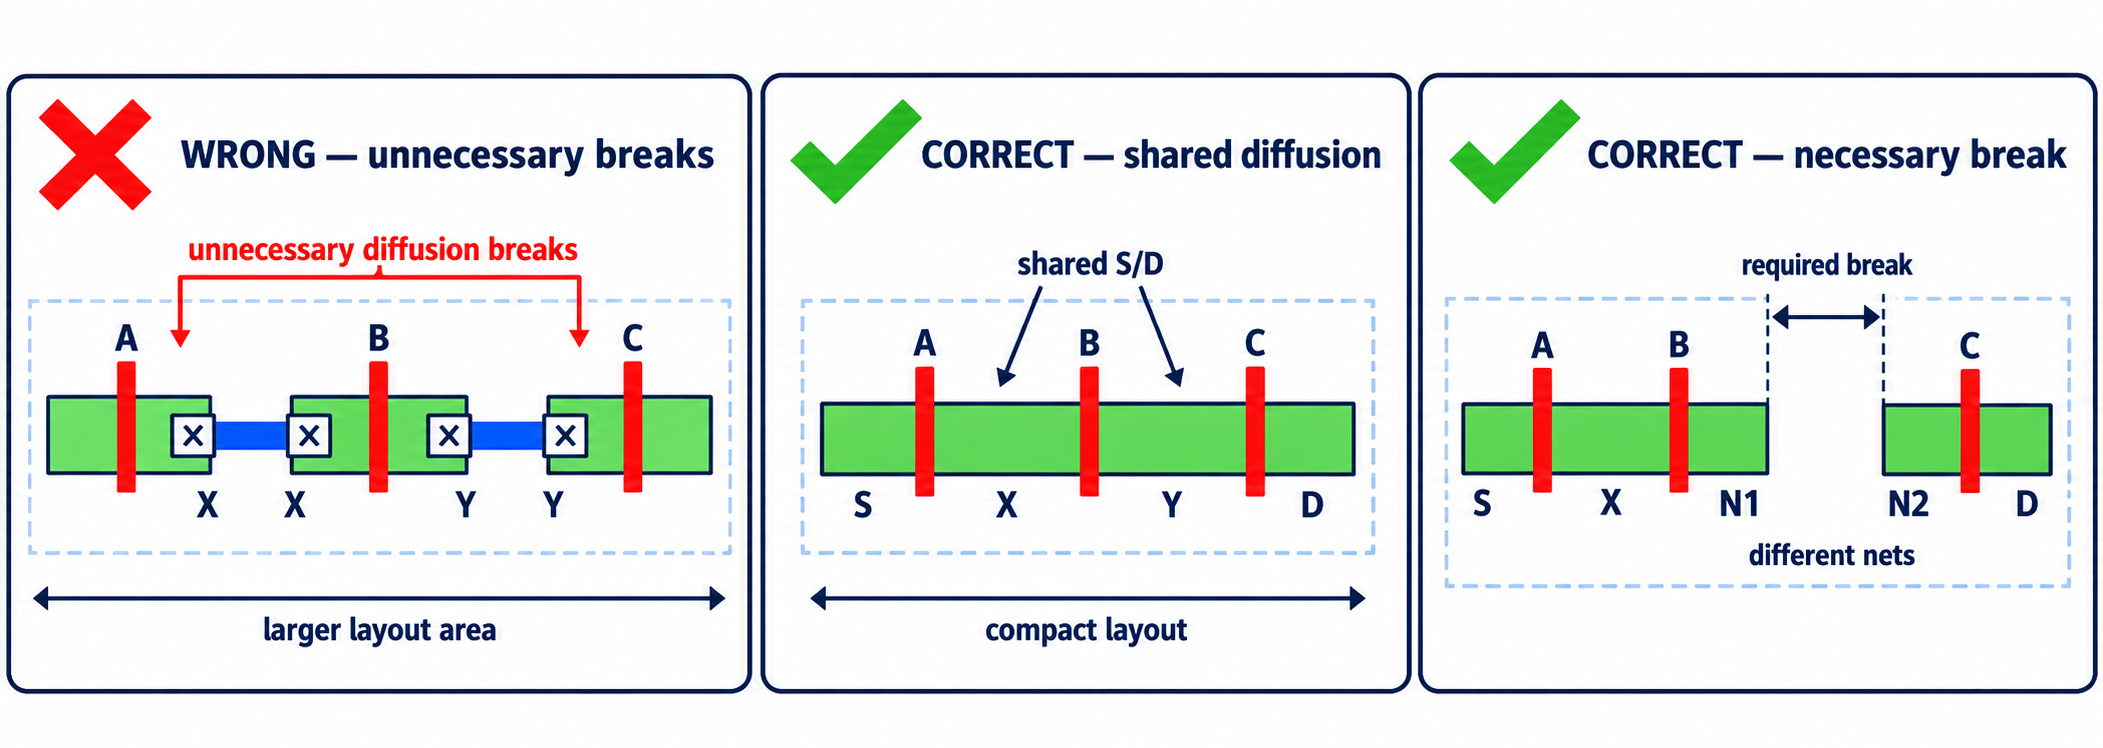
\includegraphics[width=1\linewidth]{figures/diffusion-breaks-comparison.png}
    \caption{Unneccesary Diffusion Breaks vs. Neccesary Diffusion Break}
    \label{fig:}
\end{figure}



\end{document}
